\documentclass[french]{beamer}

\usepackage[utf8]{inputenc}
\usepackage[T1]{fontenc}
\usepackage{lmodern}
\usepackage{amsmath, amssymb}

\usepackage{babel}

%CHOIX DU THEME et/ou DE SA COULEUR
%\usetheme{PaloAlto}
%\usetheme{Madrid}

\usetheme{Copenhagen}

% => il est possible, pour un thème donné, de modifier seulement la couleur
%\usecolortheme{crane}
\usecolortheme{seahorse}
%\useoutertheme[left]{sidebar}

\title{Projet collaboratif : Polen}
\subtitle{Partie Élasticité linéaire}
\author{Nabil Belahrach \& Alexandre Corizzi}
\date{Novembre 2015}
\institute{Université de Strasbourg -- U.F.R. de Mathèmatiques
et d'Informatique}

\begin{document}

\AtBeginSection[{\begin{frame}{Outline}
    \tableofcontents[hideothersubsections, pausesections] 
\end{frame}}]

\begin{frame}
  \titlepage
\end{frame}
\begin{frame}{Plan}
  \tableofcontents
\end{frame}

% ------------------------------------------------------------------------------
\section{Présentation du problème}
\begin{frame}
  \vfill
  \centering
  \begin{beamercolorbox}[sep=8pt,center,shadow=true,rounded=true]{title}
    \usebeamerfont{title}\insertsectionhead
  \end{beamercolorbox}
  \vfill
\end{frame}
% ------------------------------------------------------------------------------

\begin{frame}{Schéma de la buse}
  \begin{center}
    \begin{figure}
      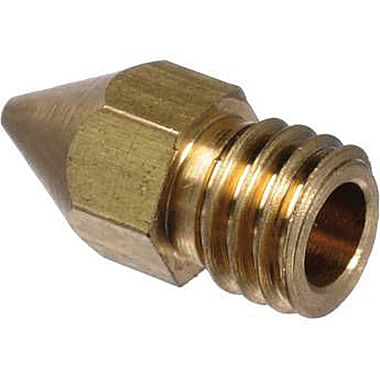
\includegraphics[scale=0.3]{images/buse.png}
      \caption{Buse reliée à la vis d'extrusion}
    \end{figure}
  \end{center}
\end{frame}

\begin{frame}{Schéma de la buse}
  \begin{minipage}{0.48\textwidth}
    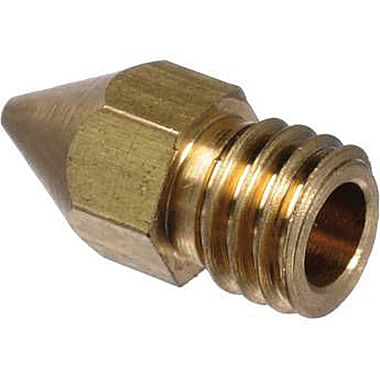
\includegraphics[scale=0.3]{images/buse.png}
  \end{minipage}
  \hspace*{\stretch{1}}
  \begin{minipage}{0.48\textwidth}
    Propriétés élastiques :
    \begin{itemize}
      \item Matériau homogéne isotrope
      \item Loi de Hooke en 3D 
    \end{itemize}
  \end{minipage}
\end{frame}


\begin{frame}{Schéma de la buse}
  \begin{minipage}{0.48\textwidth}
    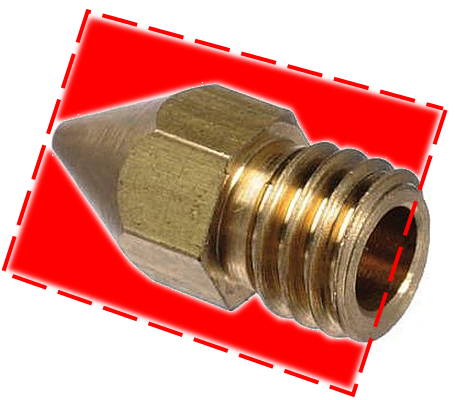
\includegraphics[scale=0.3]{images/buseCoupe.png}
  \end{minipage}
  \hspace*{\stretch{1}}
  \begin{minipage}{0.48\textwidth}
    Propriétés géométriques :
    \begin{itemize}
      \item Axisymétrique
      \item Utilisation de Coordonnées cylindriques
      \item Passage à un Problème 2D
    \end{itemize}
  \end{minipage}
\end{frame}



% ------------------------------------------------------------------------------
\section{Formulation des équations}
\begin{frame}
  \vfill
  \centering
  \begin{beamercolorbox}[sep=8pt,center,shadow=true,rounded=true]{title}
    \usebeamerfont{title}\insertsectionhead
  \end{beamercolorbox}
  \vfill
\end{frame}
% ------------------------------------------------------------------------------

\subsection{Principaux acteurs}
\begin{frame}{Déplacement et déformation}
  \begin{itemize}
    \item Vecteurs de deplacement (inconnus) : $\vec{u} \in \mathbb{R}^3 $
  \end{itemize}
  \pause
  \vspace{2pt}
  \begin{equation}
    \nabla u =  
    \left(
    \begin{array}{ccc}
      \frac{\partial u_x}{\partial x } & \frac{\partial u_x}{\partial y } & 
      \frac{\partial u_x}{\partial z }  \\
      \frac{\partial u_y}{\partial x } & \frac{\partial u_y}{\partial y } & 
      \frac{\partial u_y}{\partial z }  \\
      \frac{\partial u_z}{\partial x } & \frac{\partial u_z}{\partial y } & 
      \frac{\partial u_z}{\partial z } 
    \end{array}
    \right)
  \end{equation}

  \pause

  \vspace{2pt}
  \begin{itemize}
    \item On définit le \emph{tenseur des déformations} symétrique : 
  \end{itemize}

  \begin{equation}
    \boxed{\epsilon = \frac{1}{2} \left( \nabla u + ^{t} \nabla u \right)}
  \end{equation}

\end{frame}


\begin{frame}{Loi de Hooke}
  La buse obéit
  \begin{equation}
	\sigma &=& \lambda \cdot \mathbf{div} \vec{u} \cdot \mathbf{I} + 2 \mu\cdot\epsilon 
    \end{equation}
  \end{frame}

  \begin{frame}{Coéffiscients de Lamé}
  \end{frame}
  \subsection{Problème aux Valeurs Propres} 
  \begin{frame}
    \begin{equation}
      \- \mathbf{ - div}  \left( \sigma \left(\vec{u}\right) \right) = \lambda \cdot \vec{u}
    \end{equation}
  \end{frame}

  \begin{frame}{Changement de variables} 
  \end{frame}

% ------------------------------------------------------------------------------
  \section{Éxpérimentatiion}
  \begin{frame}
    \vfill
    \centering
    \begin{beamercolorbox}[sep=8pt,center,shadow=true,rounded=true]{title}
      \usebeamerfont{title}\insertsectionhead
    \end{beamercolorbox}
    \vfill
  \end{frame}
% ------------------------------------------------------------------------------


  \begin{frame}{Code FreeFem++}
  \end{frame}


  \end{document}
